\chapter{Nierfysiologie en osmoregulatie}\label{ch:b3:renal-osmoregulation}

De nieren filtreren per dag honderdtachtig liter plasma --- het hele
bloedvolume elk half uur --- en geven er op anderhalve liter na alles
van terug, nadat zij het ureum eruit hebben gehaald en het zout, het
zuur en het water tot op een procent hebben afgestemd op wat het
lichaam nodig heeft, en elke gram glucose hebben behouden. Een
kangoeroerat in de woestijn drinkt nooit: hij leeft van het water dat
zijn stofwisseling uit droge zaden maakt en scheidt urine uit die vijf
maal geconcentreerder is dan zeewater. Een zeevis drinkt onophoudelijk
en pompt het zout door zijn kieuwen naar buiten; een zoetwatervis
drinkt nooit en pompt zout naar binnen. Het probleem dat zij alle
oplossen is hetzelfde: de samenstelling van de vloeistof rond de cellen
constant houden terwijl eten, drinken en ademen haar verstoren, en
stikstof lozen zonder te veel water te lozen. Dit hoofdstuk behandelt
de nier van het zoogdier als uitgewerkt voorbeeld --- filtratie, de
rekenkunde van de klaring, de tegenstroomtruc die de urine
concentreert, en de hormonen die de knoppen instellen --- en daarna de
reeks oplossingen bij de dieren.

\section{Het probleem}

\begin{definition}[Osmoregulatie]\label{def:b3:renal-osmoregulation:problem}
\index{osmolariteit}\index{osmotische druk}\index{extracellulaire vloeistof}\index{osmoconformer}\index{osmoregulator}
De \emph{osmolariteit} van een oplossing is haar totale concentratie
aan opgeloste deeltjes (in osmol per liter); zij bepaalt de
\emph{osmotische druk}, $\Pi = cRT$ voor verdunde oplossingen, die
water drijft door elk membraan dat water doorlaat maar de opgeloste
stof niet. De lichaamsvloeistoffen van een zoogdier liggen rond
\qty{300}{mOsm/L} --- \qty{40}{\%} van de lichaamsmassa binnen de
cellen, \qty{20}{\%} erbuiten, de \emph{extracellulaire vloeistof}
waarvan een kwart plasma is --- en cellen zwellen of krimpen binnen
seconden als er buiten iets verandert, want hun membranen laten water
vrij door. Een \emph{osmoconformer} (de meeste ongewervelde zeedieren,
haaien) houdt zijn vloeistoffen op de osmolariteit van de zee en regelt
alleen hun samenstelling; een \emph{osmoregulator} (gewervelden,
insecten, zoetwaterdieren) houdt zijn osmolariteit constant tegenover
de omgeving, wat energie kost naar rato van het verval. De tweede taak,
aan de eerste gekoppeld, is het lozen van de stikstof uit de afbraak
van eiwit: als \emph{ammoniak} in overvloedig water (vissen), als
\emph{ureum}, oplosbaar en ongiftig maar met water nodig om het te
dragen (zoogdieren), of als \emph{urinezuur}, een pasta die vrijwel
droog wordt uitgescheiden (vogels, reptielen, insecten).
\end{definition}

\section{Het nefron en de filtratie}

\begin{definition}[Het nefron]\label{def:b3:renal-osmoregulation:nephron}
\index{nefron}\index{glomerulus}\index{proximale tubulus}\index{lis van Henle}\index{verzamelbuis}
Elke menselijke nier bevat ongeveer een miljoen \emph{nefronen}. Het
bloed komt een \emph{glomerulus} binnen, een kluwen haarvaten in het
kapsel van Bowman, wier wanden --- gevensterd endotheel,
basaalmembraan, en de spleetdiafragma's tussen de voetjes van de
podocyten --- water en elke opgeloste stof onder ongeveer \qty{60}{kDa}
doorlaten maar de eiwitten en de cellen tegenhouden. Het filtraat
stroomt door de \emph{proximale tubulus}, die twee derde van het water
en het zout en alle glucose en aminozuren terugneemt; de \emph{lis van
Henle} in en uit, die tot in het merg reikt en het concentratieverval
van de volgende paragraaf opbouwt; door de \emph{distale tubulus}, waar
het zout wordt bijgesteld; en de \emph{verzamelbuis} in, waar het
uiteindelijke watergehalte door vasopressine wordt bepaald terwijl de
buis door het merg naar het nierbekken loopt. Het bloed dat de
glomerulus verlaat komt in een tweede haarvatennet rond de tubuli, dat
opneemt wat zij terugnemen.
\end{definition}

\begin{omfigure}
\begin{tikzpicture}[every node/.style={font=\scriptsize}, >=stealth]
  % cortex/medulla background
  \fill[omDef!6] (-0.5,0) rectangle (11.5,3.6); \fill[omProp!8] (-0.5,-3.4) rectangle (11.5,0);
  \node[right, gray] at (-0.4,3.4) {schors}; \node[right, gray] at (-0.4,-3.2) {merg};
  % glomerulus
  \draw[thick, omThm, fill=omThm!20] (0.8,2.6) circle (0.55); \node[below, align=center] at (0.25,2.0) {glomerulus:\\filtratie,\\\qty{180}{L/dag}};
  % proximal tubule
  \draw[very thick, omDef] (1.35,2.6) .. controls (2.2,3.3) and (2.8,2.0) .. (3.2,2.6) .. controls (3.5,3.1) and (3.9,2.2) .. (4.2,2.6);
  \node[below, align=center] at (2.65,2.05) {proximale tubulus:\\\qty{67}{\%} van Na$^{+}$ en water,\\alle glucose, aminozuren,\\HCO$_3^-$};
  % loop of Henle
  \draw[very thick, omDef] (4.2,2.6) -- (4.2,-2.8) arc[start angle=180, end angle=360, radius=0.4] -- (5.0,2.6);
  \node[left, align=right] at (4.1,-1.0) {dalende tak:\\water verlaat};
  \node[right, align=left] at (5.1,-1.6) {stijgende tak:\\NaCl weggepompt,\\geen water};
  \node[right, align=left, omProp!80!black] at (5.1,-0.2) {\qty{25}{\%} van Na$^{+}$};
  % distal tubule
  \draw[very thick, omDef] (5.0,2.6) .. controls (5.4,3.2) and (6.0,2.0) .. (6.4,2.6) .. controls (6.8,3.1) .. (7.2,2.6);
  \node[above, align=center] at (6.0,3.1) {distale tubulus: Na$^{+}$ (aldosteron),\\Ca$^{2+}$, uitscheiding van K$^{+}$};
  % collecting duct
  \draw[very thick, omMeth!70!black] (7.2,2.6) -- (7.8,2.6) -- (7.8,-3.2);
  \node[right, align=left] at (7.9,-1.2) {verzamelbuis:\\water (vasopressine,\\aquaporine-2),\\ureum, H$^{+}$;\\\qty{1.5}{L/dag} eruit};
  \draw[->, thick, omMeth!70!black] (7.8,-3.2) -- (7.8,-3.6);
  % osmolarity scale on the right
  \foreach \y/\c in {2.6/300, 0.0/600, -1.4/900, -2.8/1200} { \node[left, omProp!80!black, font=\tiny] at (11.4,\y) {\c\ mOsm}; }
  \draw[->, omProp!80!black] (11.4,2.9) -- (11.4,-3.1); \node[above, omProp!80!black, font=\tiny, align=center] at (11.4,3.0) {osmolariteit van\\het interstitium};
\end{tikzpicture}

{\small Een \omterm{def:b3:renal-osmoregulation:nephron}{nefron} uitgelegd. Filtratie in de schors; de grote
terugname in de \omterm{def:b3:renal-osmoregulation:nephron}{proximale tubulus}; de \omterm{def:b3:renal-osmoregulation:nephron}{lis van Henle} die in het merg
duikt, waar het interstitium met de diepte zouter wordt; de
\omterm{def:b3:renal-osmoregulation:nephron}{verzamelbuis} die door dat verval terugloopt en water afstaat als
vasopressine het toelaat.}
\end{omfigure}

\begin{theorem}[Filtratie en klaring]\label{thm:b3:renal-osmoregulation:clearance}
\index{krachten van Starling}\index{glomerulaire filtratiesnelheid}\index{klaring}\index{inuline}\index{creatinine}
Het filtraat stroomt door de wand van de \omterm{def:b3:renal-osmoregulation:nephron}{glomerulus} met een snelheid
die door de \emph{\omterm{thm:b3:renal-osmoregulation:clearance}{krachten van Starling}} wordt bepaald: de
hydrostatische druk van het haarvat $P_{\text{GC}}$ duwt vloeistof naar
buiten, de hydrostatische druk in de ruimte van Bowman $P_{\text{BS}}$
en de oncotische druk van de plasma-eiwitten $\pi_{\text{GC}}$ trekken
haar terug, en
\[
\text{GFR} = K_{f}\,\bigl(P_{\text{GC}} - P_{\text{BS}} - \pi_{\text{GC}}\bigr)
\approx K_{f}\,(55 - 15 - 30)\ \unit{mmHg} = K_{f}\times \qty{10}{mmHg},
\]
de \emph{\omterm{thm:b3:renal-osmoregulation:clearance}{glomerulaire filtratiesnelheid}}, ongeveer \qty{125}{mL/min}
bij een volwassene. Voor elke stof $x$ met plasmaconcentratie $P_{x}$,
urineconcentratie $U_{x}$ en urinestroom $V$ is de \emph{klaring}
\[
C_{x} = \frac{U_{x}\,V}{P_{x}}
\]
het volume plasma dat per tijdseenheid van $x$ wordt ontdaan. Wordt $x$
vrij gefiltreerd en niet teruggenomen en niet uitgescheiden (inuline,
en bijna zo creatinine), dan is $C_{x} = \text{GFR}$; wordt het
volledig verwijderd uit het plasma dat de nier passeert
(para-aminohippuraat in lage dosis), dan is $C_{x}$ gelijk aan de
plasmastroom door de nier; een klaring onder de GFR betekent netto
terugname, erboven netto uitscheiding, en de gefiltreerde vracht $\text{GFR}
\times P_{x}$ min de uitscheiding $U_{x}V$ is de teruggenomen
hoeveelheid.
\end{theorem}
\begin{proof}
Filtratie is ultrafiltratie door een poreuze wand: de stroom is
evenredig met de netto druk erover, en de netto druk is de naar buiten
gerichte hydrostatische druk min de naar binnen gerichte hydrostatische
en oncotische druk (Starling), waarbij de oncotische druk van het
filtraat verwaarloosbaar is omdat het geen eiwit bevat. Klaring: per
tijdseenheid scheidt de nier $U_{x}V$ van $x$ uit; het plasmavolume dat
die hoeveelheid bevatte is $U_{x}V/P_{x}$. Voor een stof die alleen
wordt gefiltreerd is wat wordt uitgescheiden wat werd gefiltreerd,
$\text{GFR}\times P_{x} = U_{x}V$, waaruit $C_{x} = \text{GFR}$. Voor
een stof die geheel wordt onttrokken wordt alle $x$ in het
doorstromende plasma, $\text{RPF}\times P_{x}$, uitgescheiden, waaruit
$C_{x} = \text{RPF}$. De massabalans geeft de teruggenomen hoeveelheid.
\end{proof}

\begin{example}[Klaringen in getallen]\label{ex:b3:renal-osmoregulation:numbers}
Inuline, ingespoten tot een plasmaspiegel van \qty{1}{mg/mL},
verschijnt in de urine met \qty{125}{mg/mL} bij een stroom van
\qty{1}{mL/min}: $C = 125\times 1/1 =
\qty{125}{mL/min}$, de GFR, \qty{180}{L/dag}. Para-aminohippuraat geeft
\qty{650}{mL/min}, de plasmastroom; met een hematocriet van $0.45$ is
de bloedstroom door de nier \qty{1.2}{L/min}, een vijfde van het
hartminuutvolume voor \qty{0.5}{\%} van de lichaamsmassa, en de
filtratiefractie $125/650 = 0.19$. Ureum: plasma \qty{5}{mmol/L}, urine
\qty{300}{mmol/L} bij \qty{1}{mL/min} --- klaring \qty{60}{mL/min}, de
helft van de GFR, zodat de helft van het gefiltreerde ureum wordt
teruggenomen. Glucose: klaring nul bij normale plasmaspiegels, elk
molecuul van de \qty{180}{g} die per dag wordt gefiltreerd keert terug.
Creatinine, door spier in een constant tempo gemaakt en alleen
gefiltreerd, is de maat voor de GFR in de kliniek: halveert de GFR, dan
verdubbelt het plasmacreatinine, zonder dat er urine hoeft te worden
verzameld.
\end{example}

\begin{method}[De nierfunctie meten]\label{met:b3:renal-osmoregulation:gfr}
\index{GFR-meting}
(1) Voor een onderzoekswaarde: spuit inuline in tot een stabiele
plasmaspiegel, verzamel urine over een bekende tijd, meet beide en
bereken $UV/P$. (2) In de kliniek: meet het plasmacreatinine en schat
daaruit de GFR met een formule die voor leeftijd, geslacht en
lichaamsomvang corrigeert; die schatting bepaalt de stadia van
chronische nierschade (een GFR onder \qty{60}{mL/min} gedurende drie
maanden). (3) Toets de selectiviteit van het filter door albumine in de
urine te meten --- normaal onder \qty{30}{mg/dag}; meer betekent een
lekkende barrière, het vroegste teken van nierschade bij diabetes.
(4) Toets het concentratievermogen door een nacht lang water te
onthouden en de \omterm{def:b3:renal-osmoregulation:problem}{osmolariteit} van de urine te meten, die boven
\qty{800}{mOsm/L} hoort te liggen; niet kunnen concentreren bij een
normale GFR wijst op de \omterm{def:b3:renal-osmoregulation:nephron}{verzamelbuis} of op vasopressine.
\end{method}

\begin{omfigure}
\begin{tikzpicture}
\begin{axis}[
  width=0.68\linewidth, height=5.6cm,
  axis x line=bottom, axis y line=left,
  xmin=0, xmax=800, ymin=0, ymax=700,
  xlabel={plasmaglucose (mg/dL)}, ylabel={mg/min},
  xlabel style={font=\small, at={(axis description cs:0.5,-0.12)}, anchor=north}, ylabel style={font=\small},
  tick label style={font=\small}, xtick={0,100,200,300,400,600,800}, ytick={0,200,375,600},
  clip=false,
]
\addplot[very thick, omDef, domain=0:800, samples=2] {1.25*x};
\addplot[very thick, omMeth!70!black, domain=0:200, samples=2] {1.25*x};
\addplot[very thick, omMeth!70!black, smooth] coordinates {(200,250) (250,300) (300,340) (350,365) (400,375) (800,375)};
\addplot[very thick, omThm, domain=0:180, samples=2] {0};
\addplot[very thick, omThm, smooth] coordinates {(180,0) (250,12) (300,35) (350,72) (400,125) (800,625)};
\draw[dashed, gray] (axis cs:180,0) -- (axis cs:180,700); \node[font=\scriptsize, gray, anchor=north west] at (axis cs:185,560) {drempel};
\draw[dashed, gray] (axis cs:0,375) -- (axis cs:800,375);
\node[font=\scriptsize, omDef, anchor=south east] at (axis cs:480,620) {gefiltreerd: GFR $\times$ P};
\node[font=\scriptsize, omMeth!70!black, anchor=south west, align=left] at (axis cs:660,395) {teruggenomen:\\$T_{m} = \qty{375}{mg/min}$};
\node[font=\scriptsize, omThm, anchor=north west] at (axis cs:520,300) {uitgescheiden};
\end{axis}
\end{tikzpicture}

{\small De titratiekromme van glucose. De gefiltreerde vracht stijgt
met de plasmaspiegel; de transporteiwitten van de \omterm{def:b3:renal-osmoregulation:nephron}{proximale tubulus}
nemen alles terug tot aan hun maximum $T_{m}$; boven de drempel, bij
ongeveer \qty{180}{mg/dL} (\qty{10}{mmol/L}), stroomt glucose over in
de urine --- de suiker in de urine bij onbehandelde diabetes.}
\end{omfigure}

\section{De urine concentreren}

\begin{proposition}[De tegenstroomvermenigvuldiger]\label{prop:b3:renal-osmoregulation:countercurrent}
\index{tegenstroomvermenigvuldiging}\index{enkelvoudig effect}\index{vasopressine}\index{aquaporine}\index{hergebruik van ureum}
De \omterm{def:b3:renal-osmoregulation:nephron}{lis van Henle} bouwt een verval van \omterm{def:b3:renal-osmoregulation:problem}{osmolariteit} op van
\qty{300}{mOsm/L} aan de schors tot \qty{1200}{mOsm/L} aan de punt van
het merg, zonder dat enige cel tegen meer dan een fractie daarvan
oppompt. De dikke stijgende tak pompt NaCl uit haar vloeistof naar het
interstitium en laat geen water door, zodat zij op elke hoogte het
interstitium ongeveer \qty{200}{mOsm/L} zouter maakt dan haar eigen
inhoud --- het \emph{\omterm{prop:b3:renal-osmoregulation:countercurrent}{enkelvoudige effect}}. De dalende tak laat water
door en komt in evenwicht met het interstitium, zodat de vloeistof die
omlaag stroomt zouter wordt naarmate zij daalt en aan de bocht een
vloeistof aflevert die al geconcentreerd is, waaruit de stijgende tak
vervolgens pompt; de vloeistof die omhoog stroomt wordt op elke hoogte
verdunder dan het interstitium en verlaat de lis met \qty{100}{mOsm/L},
hypotoon. De tegenstroom zet een klein dwarseffect om in een groot
verval in de lengte: de zoutste vloeistof aan de bocht is gemaakt uit
vloeistof die al zout was, trap na trap. De \omterm{def:b3:renal-osmoregulation:nephron}{verzamelbuis} loopt daarna
door dat verval omlaag. Zonder \emph{vasopressine} (antidiuretisch
hormoon) laat haar wand geen water door en vertrekt er elk uur een
liter of meer verdunde urine; met het hormoon worden
\emph{aquaporine-2}-kanalen in het membraan aan de lumenzijde gebracht,
verlaat water de buis langs het verval het merg in, en bereikt de urine
de \omterm{def:b3:renal-osmoregulation:problem}{osmolariteit} van de punt, \qty{1200}{mOsm/L}. Ureum, uit de
binnenste buis teruggenomen en in het merg gevangen, levert de helft
van de \omterm{def:b3:renal-osmoregulation:problem}{osmolariteit} van de punt, en de vasa recta, zelf in tegenstroom,
voeren het teruggenomen water af zonder het verval weg te spoelen.
\end{proposition}

\begin{proof}[Bewijsmateriaal]
Wirz, Hargitay en Kuhn (1951) bevroren nieren van ratten en maten het
smeltpunt van de vloeistof in coupes van schors tot papil: de
\omterm{def:b3:renal-osmoregulation:problem}{osmolariteit} steeg gestaag met de diepte en bereikte aan de punt de
waarde van de urine --- het verval dat de theorie van de
tegenstroomvermenigvuldiger (Kuhn, een fysisch chemicus, 1942) had
geëist. Micropunctie van de tubuli (Gottschalk, 1959) vond daarna de
vloeistof aan de bocht van de lis hypertoon en die uit de stijgende tak
hypotoon, met de vloeistof van de \omterm{def:b3:renal-osmoregulation:nephron}{verzamelbuis} op elke hoogte gelijk
aan het interstitium wanneer vasopressine aanwezig was. De
woestijnknaagdieren met de langste lissen hadden het steilste verval en
de meest geconcentreerde urine.
\end{proof}

\begin{omfigure}
\begin{tikzpicture}[every node/.style={font=\scriptsize}, >=stealth]
  % loop
  \draw[very thick, omDef] (0,3.2) -- (0,-0.4) arc[start angle=180, end angle=360, radius=0.7] -- (1.4,3.2);
  \draw[very thick, omDef] (0.35,3.2) -- (0.35,-0.4) arc[start angle=180, end angle=360, radius=0.35] -- (1.05,3.2);
  % interstitial osmolarity bands
  \foreach \y/\c/\col in {2.8/300/10, 2.0/500/25, 1.2/700/40, 0.4/900/55, -0.4/1100/70, -1.0/1200/80} { \fill[omProp!\col, opacity=0.5] (-2.2,\y-0.4) rectangle (-0.2,\y+0.4); \node[left, font=\tiny] at (-2.25,\y) {\c}; }
  \node[left, align=right, font=\tiny] at (-2.25,3.35) {weefselvocht\\(mOsm/L)};
  % arrows: water out of descending, NaCl out of ascending
  \foreach \y in {2.4,1.6,0.8,0.0} { \draw[->, thick, omDef!70!black] (0.15,\y) -- (-0.4,\y); }
  \node[left, omDef!70!black, font=\tiny] at (-0.45,2.4) {H$_2$O};
  \foreach \y in {2.4,1.6,0.8,0.0} { \draw[->, thick, omThm] (1.25,\y) -- (1.9,\y); }
  \node[right, omThm, font=\tiny] at (1.5,2.85) {NaCl weggepompt};
  % fluid osmolarity labels inside limbs
  \node[above] at (0.17,3.25) {\qty{300}{} erin}; \node[above] at (1.22,3.25) {\qty{100}{} eruit};
  \node[font=\tiny] at (0.7,-1.35) {1200 aan de bocht};
  \node[below, align=center] at (0.2,-1.7) {dalende tak: water verlaat,\\vloeistof concentreert; stijgende tak:\\zout verlaat, vloeistof verdunt};
  % collecting duct
  \draw[very thick, omMeth!70!black] (4.2,3.2) -- (4.2,-1.4); \node[above, align=center] at (4.2,3.25) {verzamelbuis};
  \foreach \y in {2.4,1.6,0.8,0.0,-0.8} { \draw[->, thick, omMeth!70!black] (4.1,\y) -- (3.5,\y); }
  \node[right, align=left, font=\tiny] at (4.3,1.2) {met vasopressine:\\aquaporine-2 ingebracht,\\water verlaat langs\\het verval};
  \node[below, align=center] at (4.2,-1.5) {urine tot\\\qty{1200}{mOsm/L}};
  % single effect note
  \node[right, align=left] at (6.4,2.6) {het enkelvoudige effect: de stijgende tak\\houdt het interstitium $\sim\qty{200}{mOsm/L}$\\boven haar eigen vloeistof op elke hoogte;\\de tegenstroom stapelt de effecten\\tot een verval van \qty{900}{mOsm/L}\\van schors tot papil};
\end{tikzpicture}

{\small De tegenstroomvermenigvuldiger. Zout dat uit de stijgende tak
wordt gepompt maakt het interstitium hypertoon; water dat uit de
dalende tak wordt getrokken concentreert de vloeistof voordat zij de
pomp bereikt; stroming in tegengestelde richtingen stapelt een klein
dwarsverschil tot een viervoudig verval, dat de \omterm{def:b3:renal-osmoregulation:nephron}{verzamelbuis} gebruikt
om de urine te concentreren wanneer vasopressine haar voor water opent.}
\end{omfigure}

\begin{proposition}[De rekenkunde van het water]\label{prop:b3:renal-osmoregulation:water}
\index{verplicht waterverlies}\index{vrijwaterklaring}
Een lichaam dat dagelijks een vracht opgeloste stof $S$ moet
uitscheiden (ongeveer \qty{600}{mOsm}, vooral ureum en zout) bij een
maximale \omterm{def:b3:renal-osmoregulation:problem}{osmolariteit} van de urine $U_{\max}$ heeft een minimaal
urinevolume $V_{\min} = S/U_{\max}$ nodig: voor een mens
$600/1200 = \qty{0.5}{L}$ per dag, het \emph{verplichte} waterverlies,
waar de longen en de huid nog ongeveer \qty{0.9}{L} aan toevoegen.
Zeewater drinken (ongeveer \qty{1000}{mOsm/L}, vrijwel alleen zout)
levert een liter water met \qty{1000}{mOsm} zout dat moet worden
uitgescheiden; bij $U_{\max}$ kost dat $1000/1200 = \qty{0.83}{L}$
urine, maar het zout wordt samen met een vracht ureum uitgescheiden, en
de netto winst ligt dicht bij nul of is negatief: een schipbreukeling
die zeewater drinkt droogt sneller uit dan een die dat niet doet. De
\emph{\omterm{prop:b3:renal-osmoregulation:water}{vrijwaterklaring}}, $V - U_{\text{osm}}V/P_{\text{osm}}$, is het
volume water zonder opgeloste stof dat de nier per tijdseenheid aan het
lichaam toevoegt of eraan onttrekt: positief bij een waterbelasting
(verdunde urine), negatief bij uitdroging.
\end{proposition}
\begin{proof}
Opgeloste stof verlaat het lichaam alleen in de urine (zweet
daargelaten), bij hoogstens de concentratie $U_{\max}$, dus geeft
$S = U V \le U_{\max}V$ dat $V \ge S/U_{\max}$. Voor zeewater: een
liter brengt \qty{1000}{mOsm}; die uitscheiden bij \qty{1200}{mOsm/L}
kost \qty{0.83}{L}, wat \qty{0.17}{L} overlaat, nog voordat de eigen
\qty{600}{mOsm} van de dag wordt meegeteld, wier uitscheiding die rest
opsoupeert. \omterm{prop:b3:renal-osmoregulation:water}{Vrijwaterklaring}: de urine met volume $V$ en \omterm{def:b3:renal-osmoregulation:problem}{osmolariteit}
$U_{\text{osm}}$ bevat $U_{\text{osm}}V$ aan opgeloste stof, die bij de
\omterm{def:b3:renal-osmoregulation:problem}{osmolariteit} van het plasma $U_{\text{osm}}V/P_{\text{osm}}$ zou
innemen; de rest van het volume is water boven dat, aan het lichaam
onttrokken.
\end{proof}

\begin{omfigure}
\begin{tikzpicture}
\begin{axis}[
  width=0.66\linewidth, height=5.4cm,
  axis x line=bottom, axis y line=left,
  xmin=0, xmax=1300, ymin=0, ymax=12,
  xlabel={osmolariteit van de urine (mOsm/L)}, ylabel={urinevolume (L/dag)},
  xlabel style={font=\small, at={(axis description cs:0.5,-0.12)}, anchor=north}, ylabel style={font=\small},
  tick label style={font=\small}, xtick={50,300,600,1200}, ytick={0.5,2,6,12},
  clip=false,
]
\addplot[very thick, omDef, domain=50:1300, samples=100] {600/x};
\draw[dashed, gray] (axis cs:300,0) -- (axis cs:300,2); \draw[dashed, gray] (axis cs:1200,0) -- (axis cs:1200,0.5);
\node[font=\scriptsize, omDef, anchor=south west] at (axis cs:350,3.5) {$V = S/U$ met $S = \qty{600}{mOsm/dag}$};
\node[font=\scriptsize, anchor=west, align=left] at (axis cs:1210,1.7) {maximale concentratie:\\\qty{0.5}{L}};
\node[font=\scriptsize, anchor=south west] at (axis cs:60,9) {maximale verdunning (\qty{50}{mOsm/L}): \qty{12}{L}};
\end{axis}
\end{tikzpicture}

{\small Het urinevolume dat nodig is om de opgeloste stof van een dag
te dragen, tegen haar concentratie. Van de meest verdunde urine die de
nier kan maken tot de meest geconcentreerde loopt het volume over een
factor vierentwintig; vasopressine kiest het punt.}
\end{omfigure}

\section{Regeling}

\begin{definition}[De regelingen]\label{def:b3:renal-osmoregulation:controls}
\index{renine--angiotensine--aldosteronsysteem}\index{aldosteron}\index{atriaal natriuretisch peptide}\index{osmoreceptor}\index{tubuloglomerulaire terugkoppeling}
Twee grootheden worden afzonderlijk geregeld: het \emph{volume} van de
\omterm{def:b3:renal-osmoregulation:problem}{extracellulaire vloeistof}, dat een kwestie is van hoeveel natrium het
lichaam vasthoudt, en haar \emph{\omterm{def:b3:renal-osmoregulation:problem}{osmolariteit}}, die een kwestie is van
water. Volume: cellen van het juxtaglomerulaire apparaat, waar de
distale tubulus het arteriooltje van zijn eigen \omterm{def:b3:renal-osmoregulation:nephron}{glomerulus} raakt, geven
\emph{renine} af wanneer de arteriële druk of het zout in de tubulus
daalt; renine knipt angiotensine I van een plasma-eiwit, het
omzettingsenzym maakt er \emph{angiotensine II} van, dat de arteriolen
vernauwt, de dorst prikkelt en \emph{aldosteron} uit de bijnierschors
vrijmaakt, dat in de loop van uren de distale tubulus en de
\omterm{def:b3:renal-osmoregulation:nephron}{verzamelbuis} natrium doet terugnemen (via het kanaal ENaC) en kalium
doet uitscheiden. De opgerekte boezems geven \emph{natriuretisch
peptide} af, dat het omgekeerde doet. \omterm{def:b3:renal-osmoregulation:problem}{Osmolariteit}:
\emph{osmoreceptoren} in de hypothalamus voelen een stijging van
\qty{1}{\%} en maken binnen minuten vasopressine uit de achterkwab van
de hypofyse vrij, en wekken dorst op; een daling zet het af. De nier
regelt ook zichzelf: de \emph{tubuloglomerulaire terugkoppeling}
vernauwt het arteriooltje van een \omterm{def:b3:renal-osmoregulation:nephron}{nefron} waarvan de distale zoutaanvoer
te hoog is, waarmee de filtratie van elk \omterm{def:b3:renal-osmoregulation:nephron}{nefron} binnen het vermogen van
zijn tubulus blijft. En het zuur--base-evenwicht: de \omterm{def:b3:renal-osmoregulation:nephron}{proximale tubulus}
wint het gefiltreerde bicarbonaat terug, de \omterm{def:b3:renal-osmoregulation:nephron}{verzamelbuis} scheidt
protonen uit tegen een duizendvoudig verval in en loost ze gebufferd op
fosfaat en vooral als ammonium dat uit glutamine is gemaakt --- de weg
waarlangs het lichaam het zuur van een eiwitrijk dieet kwijtraakt.
\end{definition}

\begin{omfigure}
\begin{tikzpicture}[every node/.style={font=\scriptsize}, >=stealth]
  \node[draw, thick, rounded corners, fill=omThm!20, align=center] (low) at (0,0) {lage arteriële druk\\of weinig NaCl in de tubulus};
  \node[draw, thick, rounded corners, fill=omDef!20, align=center] (ren) at (3.6,0) {juxtaglomerulaire cellen\\geven renine af};
  \node[draw, thick, rounded corners, fill=omDef!20, align=center] (ang) at (7.4,0) {angiotensine I $\to$ II\\(omzettingsenzym)};
  \node[draw, thick, rounded corners, fill=omMeth!25, align=center] (ald) at (11.0,1.2) {aldosteron:\\Na$^{+}$ vastgehouden, K$^{+}$ verloren};
  \node[draw, thick, rounded corners, fill=omMeth!25, align=center] (vc) at (11.0,-0.3) {arteriolen vernauwen};
  \node[draw, thick, rounded corners, fill=omMeth!25, align=center] (th) at (11.0,-1.8) {dorst, vasopressine};
  \draw[->, thick] (low) -- (ren); \draw[->, thick] (ren) -- (ang);
  \draw[->, thick] (ang) -- (ald.west); \draw[->, thick] (ang) -- (vc.west); \draw[->, thick] (ang) -- (th.west);
  \node[draw, thick, rounded corners, fill=omProp!25, align=center] (res) at (6.8,-2.6) {volume en druk hersteld};
  \draw[->, thick] (ald.east) -- ++(0.4,0) |- (res.east); \draw[thick] (vc.east) -- ++(0.4,0); \draw[thick] (th.east) -- ++(0.4,0);
  \draw[-|, thick, omThm] (res.south) -- ++(0,-0.6) -| (low.south) node[pos=0.3, below, font=\tiny] {negatieve terugkoppeling};
  \node[draw, thick, rounded corners, fill=gray!15, align=center, font=\tiny] (anp) at (2.4,-2.6) {opgerekte boezems: natriuretisch\\peptide, het omgekeerde};
  \draw[-|, thick, gray!60!black] (anp.east) -- (res.west);
\end{tikzpicture}

{\small De lus van renine--angiotensine--aldosteron, de trage regelaar
van het natrium van het lichaam en daarmee van zijn extracellulaire
volume. Angiotensine II werkt tegelijk op de vaten, de bijnier, het
brein en de nier; natriuretisch peptide uit het opgerekte hart werkt
het tegen.}
\end{omfigure}

\begin{example}[Twee dagen]\label{ex:b3:renal-osmoregulation:two-days}
Een dag zonder water: de \omterm{def:b3:renal-osmoregulation:problem}{osmolariteit} van het plasma stijgt van $290$
naar \qty{295}{mOsm/L}, vasopressine stijgt binnen minuten, de
verzamelbuizen gaan open voor water, de urine concentreert tot
\qty{1200}{mOsm/L} en daalt tot een halve liter; de persoon heeft
dorst; het verloren volume komt vooral uit de cellen, wier water het
extracellulaire zout volgt. Een liter water in één keer gedronken: de
\omterm{def:b3:renal-osmoregulation:problem}{osmolariteit} daalt \qty{1}{\%}, vasopressine daalt binnen twintig
minuten tot nul, de buizen sluiten, en in de volgende twee uur laat de
nier een liter urine van \qty{50}{mOsm/L} door. Een bloeding van een
liter: de druk daalt, renine en vasopressine stijgen beide (volume gaat
vóór \omterm{def:b3:renal-osmoregulation:problem}{osmolariteit}), de arteriolen vernauwen, natrium en water worden
vastgehouden, en in de loop van een dag wordt het plasmavolume weer
aangevuld --- met vocht uit het interstitium en daarna uit wat er wordt
gedronken. Diabetes insipidus, het ontbreken van vasopressine of van
zijn receptor, geeft \qty{15}{L} verdunde urine per dag en een dorst
die daarbij past; nierfalen, het ontbreken van filtratie, laat een
lichaam achter dat driemaal per week door een machine moet worden
gefiltreerd, door een membraan wier klaring een fractie is van die van
twee nieren.
\end{example}

\begin{omfigure}
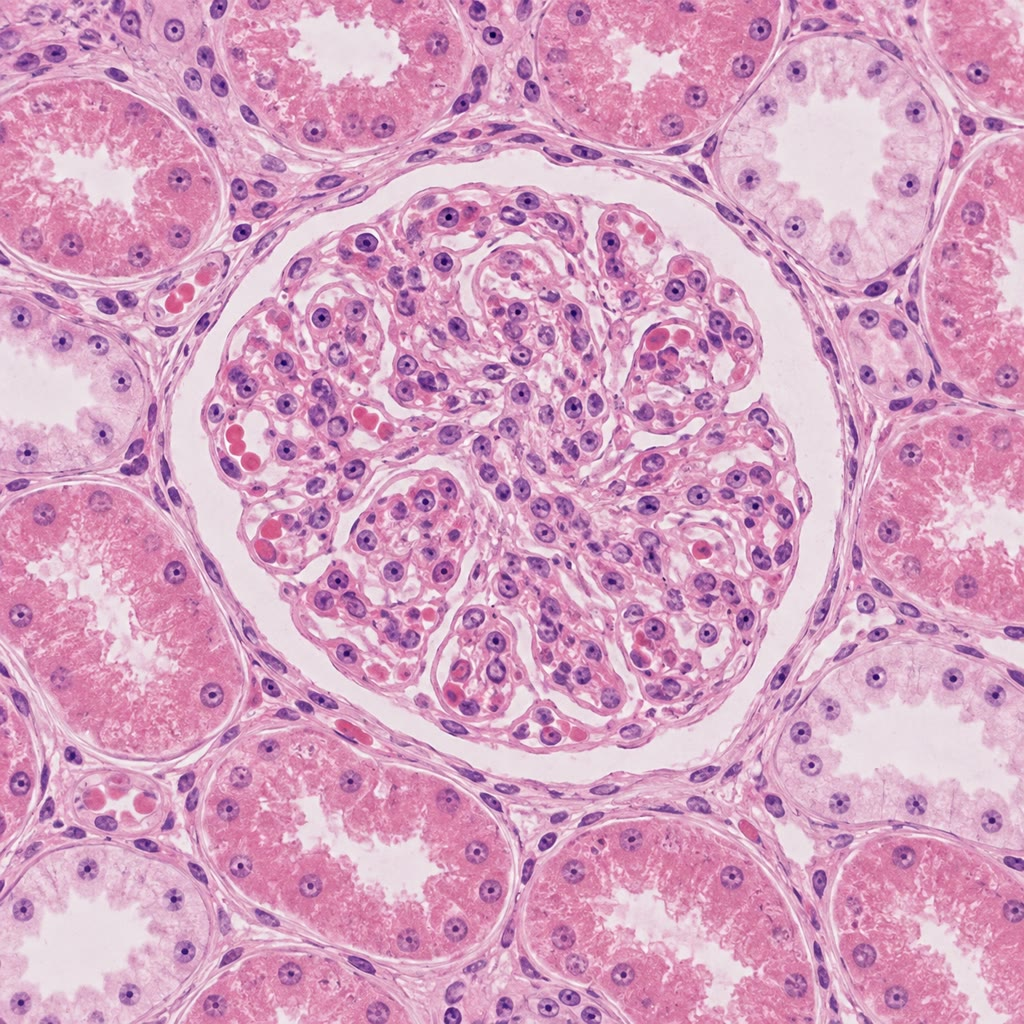
\includegraphics[width=0.46\linewidth]{images/book5/ai/b5-20-kidney-section.jpg}\hspace{0.04\linewidth}
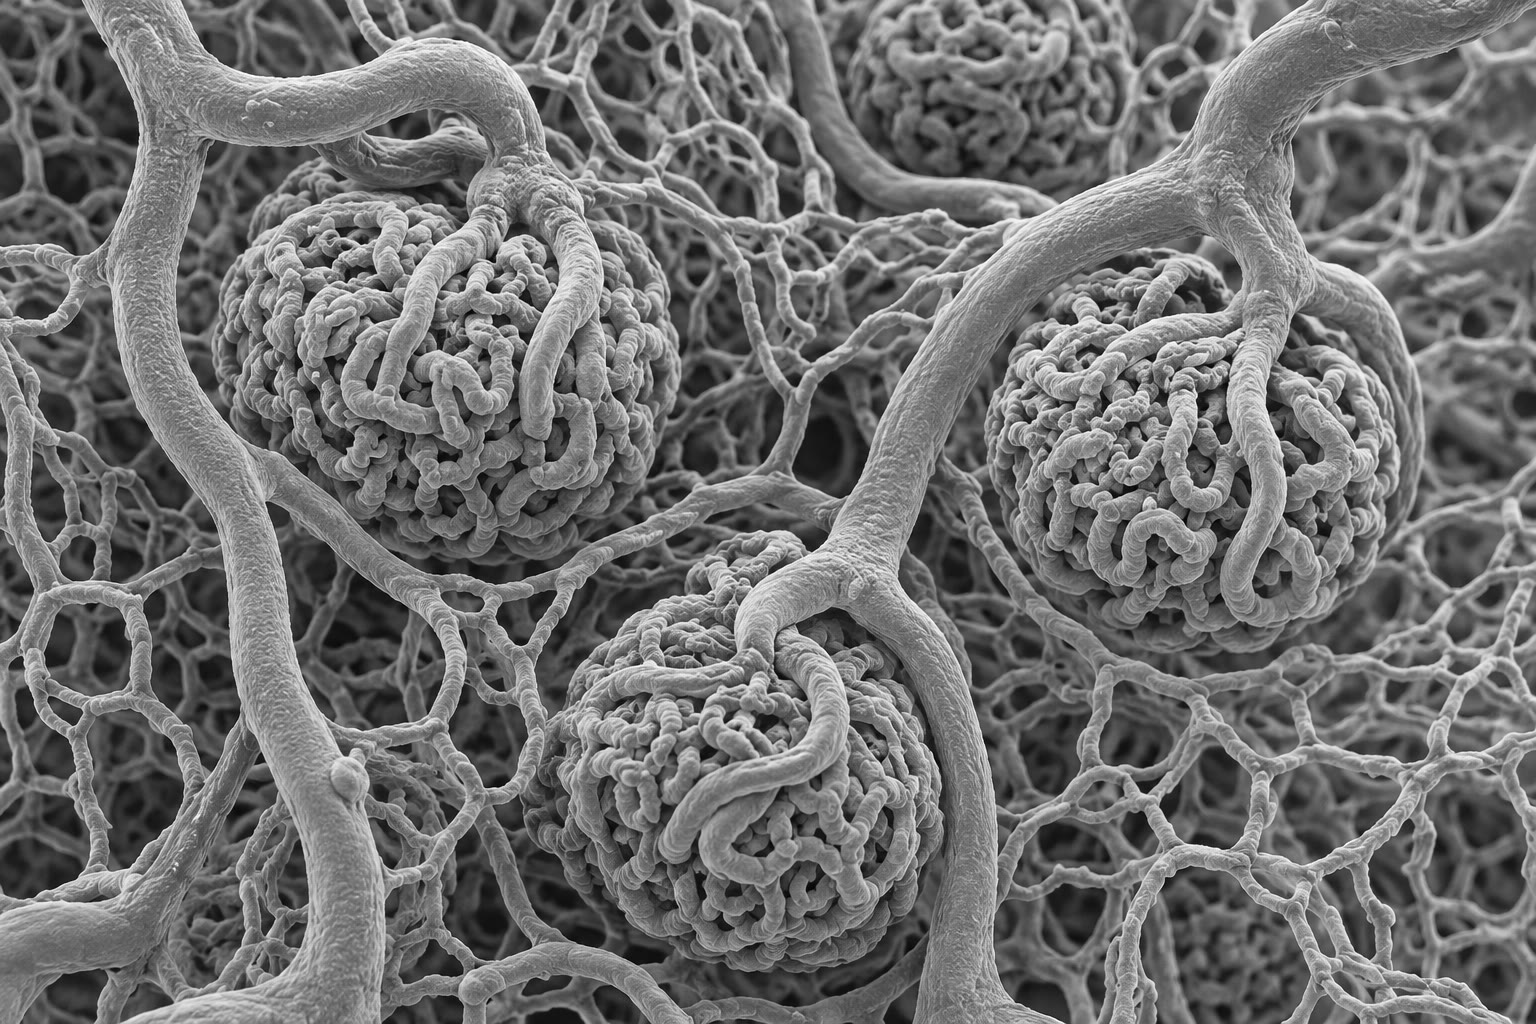
\includegraphics[width=0.46\linewidth]{images/book5/ai/b5-20-nephron-cast.jpg}

{\small Links: nierschors in doorsnede --- een \omterm{def:b3:renal-osmoregulation:nephron}{glomerulus} in zijn
kapsel tussen de doorsneden van proximale en distale tubuli. Rechts:
een vaatafgietsel van de schors, elke kluwen een \omterm{def:b3:renal-osmoregulation:nephron}{glomerulus} met zijn
aanvoerende en afvoerende vat tussen de peritubulaire haarvaten.}
\end{omfigure}

\section{Andere dieren, andere oplossingen}

\begin{definition}[Osmoregulatie bij de dieren]\label{def:b3:renal-osmoregulation:comparative}
\index{buis van Malpighi}\index{zoutklier}\index{chloridecel}\index{metabool water}\index{relatieve mergdikte}
Zoetwatervissen leven in een medium met een tiende van de \omterm{def:b3:renal-osmoregulation:problem}{osmolariteit}
van hun bloed: water stroomt door de kieuwen naar binnen, zout lekt
naar buiten, en zij scheiden overvloedige verdunde urine uit en nemen
zout actief op door de \emph{chloridecellen} van de kieuwen, zonder
ooit te drinken. Beenvissen in zee, wier bloed een derde van de
\omterm{def:b3:renal-osmoregulation:problem}{osmolariteit} van de zee heeft, verliezen water door de kieuwen, drinken
zeewater en pompen het zout naar buiten door dezelfde chloridecellen in
omgekeerde richting, terwijl zij de urine karig houden; haaien houden
hun bloed in plaats daarvan iso-osmotisch met de zee door ureum vast te
houden (en trimethylamineoxide om hun eiwitten ertegen te
stabiliseren), en lozen overtollig zout door een rectale klier.
Zeevogels en zeereptielen dragen boven de ogen \emph{zoutklieren} die
een pekel uitscheiden die tweemaal zo zout is als de zee, zodat een
albatros uit de oceaan kan drinken. Insecten filtreren door
\emph{buizen van Malpighi} die door actieve kaliumuitscheiding worden
aangedreven in plaats van door bloeddruk, en nemen in de endeldarm zo
volledig water terug dat de uitwerpselen van een woestijnkever droog
zijn. Bij de zoogdieren schaalt het concentratievermogen met de lengte
van de lissen ten opzichte van de omvang van de nier (de
\emph{relatieve mergdikte}): een bever haalt \qty{500}{mOsm/L}, een
mens \num{1200}, een kameel \num{3000}, de kangoeroerat \num{5500} ---
waardoor die kan leven van het \emph{metabole water} dat vrijkomt
wanneer zijn voedsel wordt geoxideerd, ongeveer \qty{0.6}{g} water per
gram zetmeel, met een neus die het water van elke uitgeademde teug
terugwint door tegenstroomkoeling.
\end{definition}

\begin{omfigure}
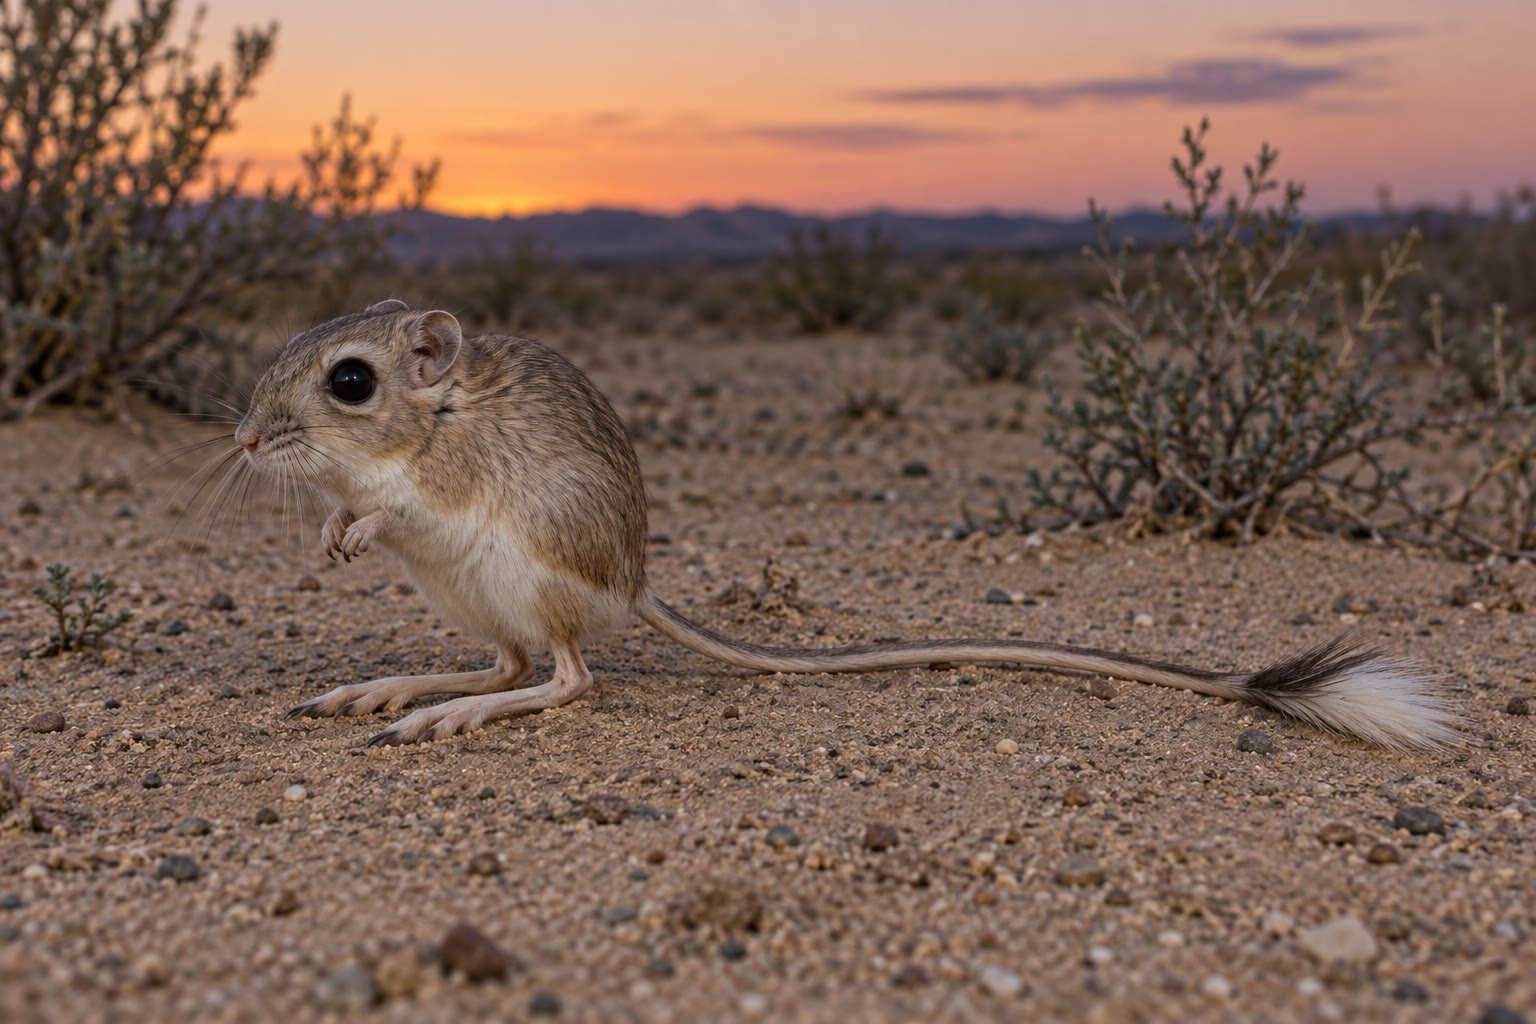
\includegraphics[width=0.56\linewidth]{images/book5/ai/b5-20-kangaroo-rat.jpg}

{\small Een kangoeroerat, die nooit drinkt: lange lissen van Henle,
urine die vijf maal zo geconcentreerd is als zeewater, een koele neus
die het water van elke ademteug laat condenseren, en een dieet waarvan
de oxidatie al het water maakt dat hij nodig heeft.}
\end{omfigure}

\begin{remark}[De nier als ontwerpprobleem]\label{rem:b3:renal-osmoregulation:design}
De nier van het zoogdier filtreert per dag veertig maal het
plasmavolume alleen om er bijna alles van terug te nemen: een
verkwistend ontwerp, waarvan de zin is dat alles filtreren en selectief
terugnemen eenvoudiger is dan elk afvalproduct dat zich zou kunnen
aandienen selectief uitscheiden. De prijs is de \qty{7}{\%} van de
rustverbranding die aan het terugpompen van natrium opgaat, en de
kwetsbaarheid is het fijne filter, dat traag bezwijkt onder hoge druk
en hoge glucose. Haar vernuft is de tegenstroomlis, een kunstgreep die
ook voorkomt in de zwemblazen van diepzeevissen, in de poten van
waadvogels en in de neuzen van woestijnknaagdieren, waarmee een klein,
betaalbaar plaatselijk verschil tot een groot wordt gestapeld ---
telkens dezelfde gedachte, dat een verval uit stroming kan worden
opgebouwd.
\end{remark}

\section{Opgaven}

\begin{exercise}[$\star$]\label{exo:b3:renal-osmoregulation:1}
Noem de segmenten van het \omterm{def:b3:renal-osmoregulation:nephron}{nefron} op volgorde en geef van elk één ding
dat het doet.
\end{exercise}

\begin{exercise}[$\star$]\label{exo:b3:renal-osmoregulation:2}
Definieer de klaring. Een stof heeft een plasmaconcentratie van
\qty{2}{mg/mL}, een urineconcentratie van \qty{100}{mg/mL} en de
urinestroom is \qty{1.5}{mL/min}. Bereken haar klaring en zeg of zij
wordt teruggenomen, uitgescheiden of geen van beide, als de GFR
\qty{120}{mL/min} bedraagt.
\end{exercise}

\begin{exercise}[$\star$]\label{exo:b3:renal-osmoregulation:3}
Waarom drinkt een zoetwatervis nooit en een zeevis onophoudelijk? Wat
doen de kieuwen in elk van beide gevallen?
\end{exercise}

\begin{exercise}[$\star$]\label{exo:b3:renal-osmoregulation:4}
Wat is het \omterm{prop:b3:renal-osmoregulation:countercurrent}{enkelvoudige effect} van de \omterm{def:b3:renal-osmoregulation:nephron}{lis van Henle}, welke tak brengt
het voort, en waarom moeten de twee takken verschillen in hun
doorlaatbaarheid voor water?
\end{exercise}

\begin{exercise}[$\star\star$]\label{exo:b3:renal-osmoregulation:5}
Druk in het haarvat van de \omterm{def:b3:renal-osmoregulation:nephron}{glomerulus} \qty{60}{mmHg}, in de ruimte van
Bowman \qty{18}{mmHg}, oncotische druk van het plasma \qty{28}{mmHg}
aan het aanvoerende eind, oplopend tot \qty{35}{mmHg} aan het
afvoerende eind. Bereken de netto filtratiedruk aan elk eind en leg uit
waarom de filtratie vóór het einde van het haarvat kan stoppen. Wat
betekent dat voor de invloed van de plasmastroom op de GFR?
\end{exercise}

\begin{exercise}[$\star\star$]\label{exo:b3:renal-osmoregulation:6}
De creatinineklaring van een patiënt is \qty{40}{mL/min}. Het
plasmanatrium is \qty{140}{mmol/L}, het urinenatrium \qty{70}{mmol/L},
de urinestroom \qty{1}{mL/min}. Bereken de gefiltreerde vracht natrium,
de uitscheiding, het teruggenomen deel en de natriumklaring.
\end{exercise}

\begin{exercise}[$\star\star$]\label{exo:b3:renal-osmoregulation:7}
Iemand eet een dieet dat \qty{900}{mOsm} opgeloste stof per dag
oplevert en kan tot \qty{1200}{mOsm/L} concentreren. Minimaal
urinevolume? Als nierziekte het maximum tot \qty{400}{mOsm/L} verlaagt,
hoeveel moet die persoon dan drinken om in evenwicht te blijven, met
\qty{0.9}{L} onmerkbaar verlies?
\end{exercise}

\begin{exercise}[$\star\star$]\label{exo:b3:renal-osmoregulation:8}
Voorspel het urinevolume en de \omterm{def:b3:renal-osmoregulation:problem}{osmolariteit}, het plasmanatrium en de
mate van dorst bij (a) diabetes insipidus, (b) ongepaste afgifte van
vasopressine door een \omterm{def:b3:cancer-biology:hallmarks}{tumor}, (c) overmaat aan \omterm{def:b3:renal-osmoregulation:controls}{aldosteron}, (d) een week
lang een dieet zonder zout.
\end{exercise}

\begin{exercise}[$\star\star$]\label{exo:b3:renal-osmoregulation:9}
Bereken de \omterm{prop:b3:renal-osmoregulation:water}{vrijwaterklaring} voor urine van \qty{100}{mOsm/L} bij
\qty{6}{mL/min} en voor urine van \qty{1000}{mOsm/L} bij
\qty{0.6}{mL/min}, met plasma op \qty{300}{mOsm/L}. Duid beide.
\end{exercise}

\begin{exercise}[$\star\star\star$]\label{exo:b3:renal-osmoregulation:10}
Modelleer de lis als $n$ trappen waarin de stijgende vloeistof op elke
trap \qty{200}{mOsm/L} onder het interstitium ligt en de dalende
vloeistof eraan gelijk is, met een vloeistof die met \qty{300}{mOsm/L}
binnenkomt. Beredeneer dat de \omterm{def:b3:renal-osmoregulation:problem}{osmolariteit} aan de bocht in de
stationaire toestand $300 +
200n$ kan naderen, zodat het verval wordt begrensd door de lengte van
de lis en door het \omterm{prop:b3:renal-osmoregulation:countercurrent}{enkelvoudige effect} van de pomp, en zeg wat $n$
fysiek bepaalt.
\end{exercise}

\begin{exercise}[$\star\star\star$]\label{exo:b3:renal-osmoregulation:11}
Een kangoeroerat eet per dag \qty{5}{g} droog zaad, voor \qty{80}{\%}
zetmeel, geoxideerd tot CO$_{2}$ en water (\qty{0.6}{g} water per gram
zetmeel). Hij moet per dag \qty{3}{mOsm} opgeloste stof uitscheiden bij
\qty{5500}{mOsm/L}, en verliest per dag \qty{1.5}{g} water door
verdamping uit een neus die \qty{70}{\%} van het water in zijn adem
terugwint. Maak zijn waterbalans op en zeg of hij het zonder drinken
redt.
\end{exercise}

\begin{exercise}[$\star\star\star$]\label{exo:b3:renal-osmoregulation:12}
Bij dialyse stroomt bloed langs de ene kant van een membraan en
dialysaat langs de andere, in tegenstroom. Leg uit waarom tegenstroom
meer klaart dan gelijkstroom, schat de klaring van een machine die
ureum uit \qty{300}{mL/min} bloed haalt met \qty{70}{\%} rendement, en
vergelijk met twee nieren over een week als de machine driemaal per
week vier uur draait.
\end{exercise}

\section{Vraagstuk: achttien emmers per dag}

\begin{problem}[{Weekendvraagstuk --- het filtraat van een dag gevolgd
van de glomerulus tot de blaas: de drukken van Starling, de klaringen
van vier stoffen, de glucosedrempel, de waterbalans van maximale
verdunning tot zeewater, en het evenwicht van een woestijnknaagdier,
eindigend bij de GFR, het verplichte urinevolume en het netto water dat
een liter zeewater oplevert}]
\label{pb:b3:renal-osmoregulation:1}
Gegevens: $K_{f} = \qty{12.5}{mL/min/mmHg}$; $P_{\text{GC}} = \qty{55}{mmHg}$,
$P_{\text{BS}} = \qty{15}{mmHg}$, $\pi_{\text{GC}} = \qty{30}{mmHg}$.
Plasma: inuline \qty{0.5}{mg/mL}, creatinine \qty{0.01}{mg/mL}, ureum
\qty{5}{mmol/L}, glucose \qty{5}{mmol/L}, para-aminohippuraat
\qty{0.02}{mg/mL}, Na$^{+}$ \qty{140}{mmol/L}, \omterm{def:b3:renal-osmoregulation:problem}{osmolariteit}
\qty{290}{mOsm/L}. Urinestroom \qty{1}{mL/min}: inuline \qty{62.5}{mg/mL},
creatinine \qty{1.3}{mg/mL}, ureum \qty{250}{mmol/L}, glucose $0$,
para-aminohippuraat \qty{13}{mg/mL}, Na$^{+}$ \qty{100}{mmol/L},
\omterm{def:b3:renal-osmoregulation:problem}{osmolariteit} \qty{600}{mOsm/L}. Hematocriet $0.45$. Glucose $T_{m} =
\qty{375}{mg/min}$ (\qty{2.1}{mmol/min}). Opgeloste stof per dag
\qty{600}{mOsm}; $U_{\max} = \qty{1200}{mOsm/L}$, $U_{\min} = \qty{50}{mOsm/L}$;
onmerkbaar verlies \qty{0.9}{L/dag}; zeewater \qty{1000}{mOsm/L}.

\medskip
\noindent\textbf{Deel I --- Het filter.}
\begin{enumerate}
  \item Bereken de netto filtratiedruk en de GFR.
  \item Reken de GFR om naar liter per dag. Hoe vaak wordt het
        plasmavolume (\qty{3}{L}) gefiltreerd?
  \item Bereken de inulineklaring en vergelijk haar met de GFR. Bereken
        de creatinineklaring; waarom is die iets groter?
  \item Bereken de klaring van para-aminohippuraat (de plasmastroom
        door de nier), de bloedstroom door de nier en de
        filtratiefractie.
  \item Het afvoerende arteriooltje vernauwt, waardoor $P_{\text{GC}}$
        tot \qty{60}{mmHg} stijgt. Nieuwe GFR? Waarom verlagen middelen
        die angiotensine II blokkeren de GFR een weinig in een gezonde
        nier en beschermen zij een diabetische?
  \item Er verschijnt \qty{3}{g/dag} eiwit in de urine. Welke laag van
        het filter heeft gefaald, en wat gebeurt er met de oncotische
        druk van het plasma en met de weefsels als dit aanhoudt?
\end{enumerate}

\medskip
\noindent\textbf{Deel II --- De verwerking.}
\begin{enumerate}[resume]
  \item Ureum: gefiltreerde vracht, uitscheiding, teruggenomen deel en
        klaring.
  \item Natrium: gefiltreerde vracht per dag in mol en in gram,
        uitscheiding, en het teruggenomen deel. Hoeveel kilogram zout
        zou er in een dag verloren gaan als er niets werd teruggenomen?
  \item Glucose: gefiltreerde vracht in mmol/min en in gram per dag;
        wordt er iets uitgescheiden? Bij welk plasmaglucose bereikt de
        gefiltreerde vracht $T_{m}$ (de drempel)?
  \item Een diabetespatiënt heeft een plasmaglucose van
        \qty{20}{mmol/L}. Uitgescheiden glucose per minuut en per dag
        in gram, en het extra urinevolume als elke \qty{300}{mOsm}
        glucose \qty{1}{L} meedraagt bij de heersende concentratie.
        Verklaar de dorst en het gewichtsverlies bij onbehandelde
        diabetes.
  \item Het terugnemen van natrium kost één ATP per drie Na$^{+}$.
        Hoeveel mol ATP per dag besteedt de nier aan natrium, en
        hoeveel kilojoule (\qty{50}{kJ/mol})? Vergelijk met
        \qty{7}{MJ/dag} in rust.
  \item Leg uit waarom de nier filtreert en terugneemt in plaats van
        elk afvalproduct uit te scheiden, in termen van wat de tubulus
        zou moeten herkennen.
\end{enumerate}

\medskip
\noindent\textbf{Deel III --- Water.}
\begin{enumerate}[resume]
  \item De osmolaire klaring $U_{\text{osm}}V/P_{\text{osm}}$ uit de
        gegevens, en de \omterm{prop:b3:renal-osmoregulation:water}{vrijwaterklaring}. Spaart de persoon water of
        loost hij het?
  \item Minimaal urinevolume voor de opgeloste stof van een dag;
        maximaal (bij $U_{\min}$); de totale dagelijkse waterbehoefte
        bij het minimum, met het onmerkbare verlies.
  \item Er wordt een liter zeewater gedronken. Hoeveel urine is er
        nodig om het zout ervan bij $U_{\max}$ uit te scheiden, en wat
        is de netto waterwinst voordat de eigen opgeloste stof van de
        dag wordt meegeteld? En daarna?
  \item Vasopressine ontbreekt (diabetes insipidus) en de urine blijft
        op $U_{\min}$. Dagelijks urinevolume voor dezelfde opgeloste
        stof, en het water dat dagelijks moet worden gedronken om in
        evenwicht te blijven.
  \item Bier van \qty{20}{mOsm/L}: hoeveel kan er per dag worden
        gedronken voordat de nier, bij $U_{\min}$, het water niet meer
        kan uitscheiden? (Water boven wat de opgeloste stof bij
        $U_{\min}$ kan dragen, hoopt zich op.)
  \item Na een nacht zonder water is de \omterm{def:b3:renal-osmoregulation:problem}{osmolariteit} van het plasma
        \qty{298}{mOsm/L}. Met hoeveel procent is zij gestegen, en wat
        doet de hypothalamus? Schat het watertekort als het totale
        lichaamswater \qty{42}{L} bedraagt en de opgeloste stof
        onveranderd is.
  \item Leg uit waarom een marathonloper die \qty{6}{L} water drinkt
        terwijl hij zout uitzweet een gevaarlijk laag plasmanatrium kan
        krijgen, en wat de nier zou moeten doen om dat te voorkomen.
\end{enumerate}

\medskip
\noindent\textbf{Deel IV --- De woestijn.}
\begin{enumerate}[resume]
  \item Een kangoeroerat scheidt per dag \qty{3}{mOsm} uit bij
        \qty{5500}{mOsm/L}. Urinevolume? Vergelijk met het volume dat
        een menselijke nier voor dezelfde opgeloste stof bij haar eigen
        maximum nodig zou hebben.
  \item Zijn voedsel levert per dag \qty{2.4}{g} \omterm{def:b3:renal-osmoregulation:comparative}{metabool water} en hij
        verliest \qty{1.6}{g} door ademen en \qty{0.3}{g} in de
        ontlasting. Maak de balans op met de urine van vraag 20.
  \item Een kameel concentreert tot \qty{3000}{mOsm/L} en verdraagt het
        verlies van \qty{25}{\%} van zijn lichaamswater. Hoeveel kan
        een kameel van \qty{500}{kg} met \qty{65}{\%} water verliezen,
        en hoeveel dagen dekt dat bij een verlies van \qty{5}{L/dag}?
  \item Een zeevogel eet per dag \qty{200}{g} vis en drinkt
        \qty{100}{mL} zeewater, waarmee hij \qty{150}{mmol} NaCl
        binnenkrijgt. Zijn \omterm{def:b3:renal-osmoregulation:comparative}{zoutklier} scheidt uit bij \qty{800}{mmol/L}.
        Hoeveel pekel maakt hij, en waarom is de klier hiervoor beter
        dan de nier (die bij vogels maar tot \qty{600}{mOsm/L}
        concentreert)?
  \item Een zoetwatervis van \qty{100}{g} wint per dag \qty{30}{\%} van
        zijn lichaamsmassa aan water door zijn kieuwen. Hoeveel urine
        moet hij maken, bij welke \omterm{def:b3:renal-osmoregulation:problem}{osmolariteit} ten opzichte van zijn
        bloed, en wat zou er zonder actieve opname met zijn zout
        gebeuren?
  \item Vat samen: de GFR (vraag~1), het verplichte urinevolume
        (vraag~14), en het netto water uit een liter zeewater nadat de
        opgeloste stof van de dag is meegeteld (vraag~15).
\end{enumerate}
\end{problem}
